
\usetikzlibrary{arrows.meta, positioning}

\begin{figure*}

    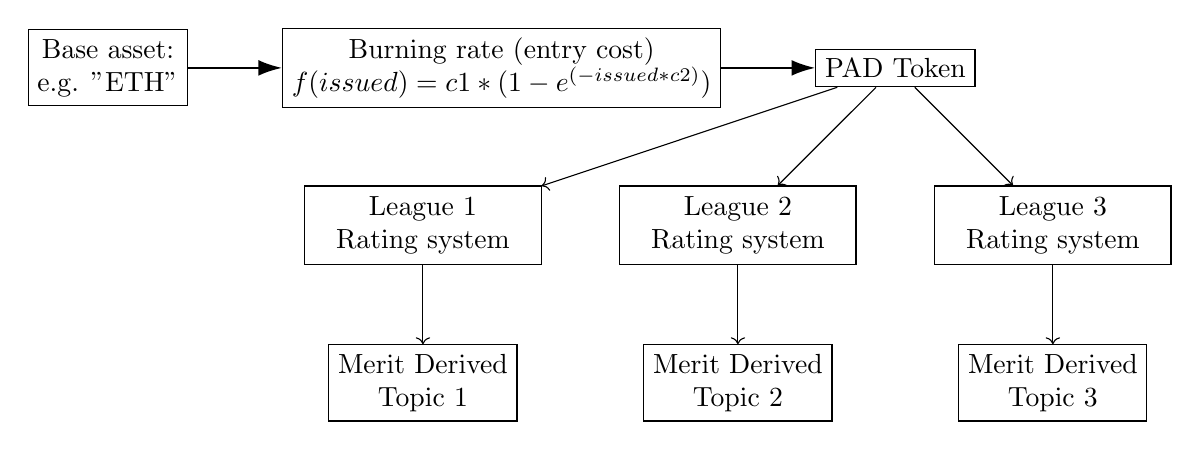
\begin{tikzpicture}[
        node distance=2cm,
        every node/.style={draw, align=center},
        arrow/.style={-{Latex[length=3mm, width=2mm]}, thick}
        ]


        % Single block for the game

        % Nodes
        \node (Competence_A) {Base asset: \\ e.g. "ETH"};
        \node[right of=Competence_A, , xshift=3cm]  (A_token) {Burning rate (entry cost)\\ $f(issued)=c1*(1-e^{(-issued*c2)})$};
        % \node[above of=A_token]  (DAO_origin) { DAO "A"};
        % \node[above of=DAO_origin] (Multisig) {Multisig M of N};
        \node[right of=A_token, xshift=3cm] (exchanger) {PAD Token};
        % \node[below of=exchanger, xshift=2cm] (Competence_B) {Ranking System B};
        % \node[above of=Competence_B]  (B_token) {Gov. Token "B"};
        % \node[above of=B_token]  (DAO_B) { DAO "B" };
        \foreach \x in {1,...,3} {
                \node[draw, rectangle, minimum width=3cm, minimum height=1cm] (P-\x) at (\x*4, -2) {};
                % Add "Rank X" text inside each block
                \node[minimum width=3cm, minimum height=1cm] at (\x*4, -2) {League \x \\ Rating system};
                \node[below of=P-\x]  (MAO-\x) {Merit Derived \\ Topic \x};


            }
        % Connect participants to the game
        \foreach \x in {1,...,3}
            { \draw[->] (exchanger) -- (P-\x);
                \draw[->] (P-\x) -- (MAO-\x);}
        \draw [arrow] (Competence_A) -- (A_token);
        % \draw [arrow] (A_token) -- (DAO_origin);
        % \draw [arrow] (DAO_origin) -- (Multisig);
        % \draw [arrow] (A_token) -- (exchanger);
        \draw [arrow] (A_token) -- (exchanger);
        % \draw [arrow] (exchanger) -- (Competence_B);
        % \draw [arrow] (Competence_B) -- (B_token);
        % \draw [arrow] (B_token) -- (DAO_B);
        % \draw [arrow] (DAO_B) -- (Multisig);






    \end{tikzpicture}
    \caption{Diagram illustrating the derivation path for base assets in to subjective merit defined values. The burn rate is defined as a function of the amount of PAD token issued, and is used to calculate price at which PAD can be purchased. PAD can be used to create and acquire a derivative token trough autonomous competence identification framework proposed in \cite{PeerskyACID2024}.}
    \label{fig:dao-composition}
\end{figure*}